
\renewcommand{\P}{Pr}

%\begin{figure}
%\begin{center}
%	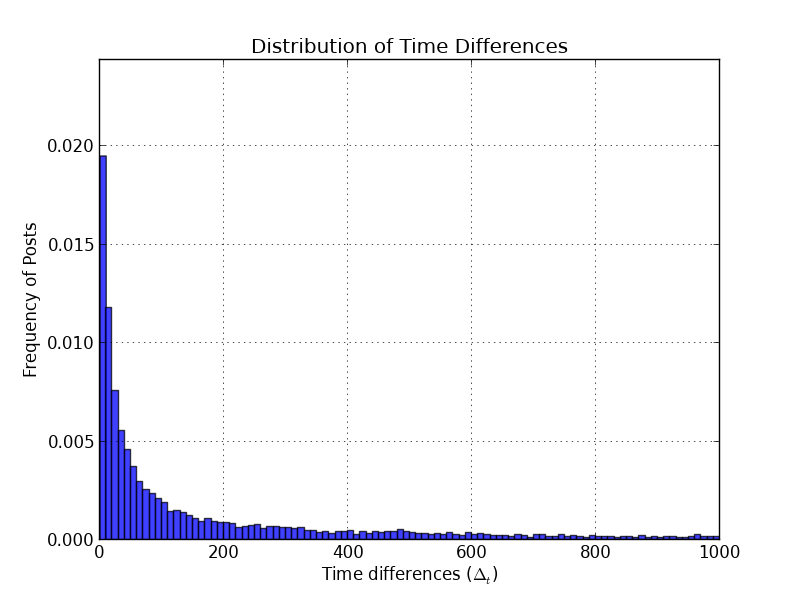
\includegraphics[width=0.8\textwidth]{diagrams/time_dist.png}
%\end{center}
%\caption{Time distribution for a subset of 97 threads}\label{fig:time_dist}
%\end{figure}
%
\begin{table}
\begin{center}
\begin{tabular}{l l}
	\hline
Notation	&	Description		\\
	\hline
$P$			&	List of posts. \\
$V$			&	List of visits.\\
$T$			&	A thread's $T$-score. \\
	$T_\text{max}$	&	A thread's maximum $T$-score. \\
$t(\post)$	&	Timestamp of the post.\\
	\hline
\end{tabular}
\end{center}
	\caption{Notation used for evaluation metrics}
\end{table}


One of the contributions of this project was also to come up with a good metric 
for measuring the performance of a model that performs predictions. 

Our metric has to be different from traditional methods of measuring 
performance. One example of such a measure is Mean Average Percentage Error 
(MAPE), which we use to measure the performance of the learnt model. This value 
is given by
\[
	\frac{1}{|P|}\sum^{|P|}_{t=1}\left|\frac{f(\X_t) - \dt}{\dt}\right|
\]
where $A_i$ is the actual value, and $F_i$ is the forecasted value for the 
instance $i$. Realistically, the model would not be able to come into contact 
with every possible window, since chances are it will make an error that causes 
 %explain error in a new section (before this one) ?
it to visit a thread late, causing it to miss two posts or more. This value does 
not reflect how well the model will do in a real-time setting, but gives an idea 
of how far off the model is given a window.

In such measures, the performance of the model is measured on an instance by 
instance basis. To give a concrete example, say we are attempting to predict 
stock prices. Given the feature vector as input, we get an estimate of what the 
stock prices will be for, say, the next day. We can then measure the absolute 
difference between what was predicted and the actual amount, and evaluate the 
model based on that.

In our case, we want to know how long it takes before any post made will be 
retrieved by the crawler. We also want to ensure that the model does not choose 
to make too many requests. The rest of the chapter explains in detail how we 
came up with our metric, its advantages and limitations.

\section{Potential errors}
To be thorough, let us also enumerate the types of errors that a model making 
predictions could encounter.

The model can potentially make a prediction such that the next visit comes 
before the arrival of the next post. The predictions being made are the $\dt$ 
between the posts, rather than the visitation times, hence, it is possible for 
the model to make a prediction that occurs before the current time. An erroneous 
prediction can also cause the crawler to come in before the next post (two, or 
more, visits, but nothing new fetched). Errors of this type waste bandwidth, 
since the crawler will make an unnecessary visit to the page.

Another type of error would have the prediction causing the next visit to come 
some time after a post. Since most predictions are almost never fully accurate, 
there will be some time between the post is made and the page is fetched. These 
errors are still relatively acceptable, but the time difference between the post 
arriving and the visit should be minimised. The visit could also come more than 
one post later. Errors of this kind incur a penalty on the freshness of the 
data, more so than the after one post, especially if the multiple posts are far 
apart time-wise.
%include diagrams

\section{$T$-score, and the Visit/Post ratio}

\begin{figure}
	\begin{center}
	\input{diagrams/t_score_diag}
	\caption{An example of a series of events used in our evaluation.}
	\end{center}
\end{figure}

We also want to know the \emph{timeliness} of the model's visits.  
\outcite{Yang2009} has a metric for measuring this. Taking $\Delta t_i$ as the 
time difference between a post $i$ and it's download time, the timeliness of the 
algorithm is given by
\[
	T = \frac{1}{|P|} \sum^{|P|}_{i=1}\Delta t_i
\]

A good algorithm would give a low $T$-score. However, a crawler that hits the 
site repeatedly performs well according to this metric. The authors account for 
this by setting a bandwidth (fixed number of pages per day) for each iteration 
of their testing. In our experimental results, we also take into account the 
number of page requests made in comparison to the number of posts. %ratio?

%\begin{align*}
%	\begin{array}{l@{\mskip\thickmuskip}l}
%	Pr_{miss} &=  \dfrac{%
%		\sum^{N-k}_{i=1} \left[\Theta_{ref\_hyp} (i,k)\right]%
%	}{%
%		\sum^{N-k}_{i=1} \left[\Delta_{ref} (i,k)\right]%
%	}\\
%	 & \\
%	Pr_{fa} &= \dfrac{%
%		\sum^{N-k}_{i=1} \left[\Psi_{ref\_hyp} (i,k)\right]%
%	}{N-k}
%	\end{array}
%	\begin{array}{l@{\mskip\thickmuskip}l}
%		\Delta_{ref}(i,k) &= \left\{ \begin{array}{l l}
%				1, & \text{if }r(i,k) > 0 \\
%				0, & \text{otherwise} 
%		\end{array} \right.\\
%		\Theta_{ref\_hyp}(i,k) &= \left\{ \begin{array}{l l}
%				1, & \text{if ends with post} \\
%				0, & \text{otherwise} 
%		\end{array} \right.\\
%		\Psi_{ref\_hyp}(i,k) &= \left\{ \begin{array}{l l}
%				1, & \text{if ends with visit}\\
%				0, & \text{otherwise} 
%		\end{array} \right.\\
%	\end{array}
%\end{align*}
%Split the $Pr_{error}$ measure into 3 parts:
%
%Probability of having visits before the first post in the window.
%Probability of having more visits than posts after the first post.
%Probability of having more posts than visits after the first post.

%Viewing the posts made during the thread's lifetime as segmentations of the 
%thread, and the visits made as hypotheses of where the segmentations are, we 
%use the $\prerror$ metric from \outcite{Georgescul2009} as a measure of how 
%close the predictions are to the actual posts. An example can be seen in Figure 
%\ref{prerror}.

%Function that gives me:
%
%Increase in visit to post ratio		increase
%Increase in interval				increase
%Increase between post and visit		increase
%(0,$\infty$ or 1)
%
%Increase between visit and visit	decrease
%($\infty$ or 1,0)
%Increase between post and post		increase
%(0,$\infty$ or 1)
%
%\[
%	\begin{array}{l l}
%	T = \dfrac{%
%		\sum_{e=1}^{|E|-1} \Psi(e_t,e_{t+1}) %
%	}{|E|-1} &
%		\Psi(e_t,e_{t+1}) = \left\{\begin{array}{l l}
%				1-e^{-(e_{t+1} - e_t)}	& \text{if post,visit}\\
%				e^{-(e_{t+1} - e_t)}			& \text{if visit,visit}\\
%		\end{array}\right.
%\end{array}
%\]

\section{Normalising the $T$-score and Visit/Post ratio}
We normalise the $T$-score to get a comparable metric across all the threads. In 
order to do this, we consider again the thread posts and visits as a sequence of 
events. We then define the \emph{lifetime}, denoted as $l$, of the thread as the 
time between the first post and the last post. Any visits that occur after the 
last post are ignored.

We then consider the worst case in terms of timeliness, or misses. This would be 
the case where the visit comes at the end, at the same time as the post. So we 
get a value $T_{\max}$ and $P_{\text{miss}}$ such that
\begin{align*}
	\P_{\text{miss}} &= \frac{T}{T_{\max}}\\
							  &= \dfrac{T}{\left(
					\dfrac{%
			\sum_\post (\max_{\post'}t(\post') - t(\post))}{|P|}\right)} \\
					&= \dfrac{|P| \cdot T}{%
		\sum_\post (\max_{\post'}t(\post') - t(\post))}
\end{align*}


An example can be viewed in Figure \ref{fig:norm_t_score}. Assuming that there 
are no posts before $\post_1$ here, we simply take the usual $T$-score value to 
get $T_\text{max}$
\begin{figure}
\begin{center}
\input{diagrams/norm_t_score_diag}
	\end{center}
\caption{An example of calculating $T_\text{max}$. A visit is assumed at the 
same time as the final post made, and the usual $T$-score metric is 
calculated}\label{fig:norm_t_score}
\end{figure}
It is difficult to consider the worst case in terms of false alarms, or visits 
that retrieve nothing. There could be an infinite number of visits made if we 
are to take the extreme case. In order to get around this, we consider discrete 
time frames in which a visit can occur. Since for this dataset, our time 
granularity is in terms of minutes, we shall use minutes as our discrete time 
frame.
With this simplified version of our series of events, we can then imagine a 
worst-case performing revisit policy that visits at every single time frame.  
Here, we assume all quantities are measured in terms of minutes. This gives us
\[
	\P_{\text{FA}} = \frac{|V|}{(\max_{\post}t(\post)) - |P|}
\]
where $l$ is in units of:our specified discrete time frame. Figure 
\ref{fig:norm_fa_score} shows an example of how $\P_{\text{FA}}$ is calculated.

\begin{figure}
\begin{center}
	\input{diagrams/fa_diag}
\end{center}
\caption{An example of calculating the maximum number of visits given a thread. 
The ratio between the number of visits predicted and the number of visits to the 
thread, and is used as $\P_{\text{FA}}$}
\label{fig:norm_fa_score}
\end{figure}


With these two normalised forms of the original metrics, we can use a weighted 
mean to give a weighted combined form of the two error rates, 
$\P_{\text{error}}$:
\[
	\P_{\text{error}} = \alpha\P_{\text{FA}} + (1-\alpha)\P_{\text{error}}
\]


In the following sections, we will discuss the results of our experiments with 
the various algorithms found in the previous chapter, and measure their 
effectiveness using their $T$-scores and Visit/Post ratio, and comparing them 
using the  $\P_{\text{error}}$ metric.

